\documentclass[aspectratio=169]{beamer}
\usetheme{metropolis}
\title{E4E Soldering Workshop}
\institute{Engineers for Exploration, UC San Diego}
\date{December 4, 2023}
\logo{
\includegraphics[height=.65cm,keepaspectratio]{e4e_logo_350x136.png}}
\setbeamertemplate{caption}[numbered]

\usepackage{graphicx}
\usepackage{hyperref}
\begin{document}
\maketitle
\begin{frame}{Obligatory Meme}
    \centering
    
\includegraphics[height=0.8\textheight]{soldering_meme.jpg}
\end{frame}
\begin{frame}{Applicable Standards}
    \begin{itemize}
        \item \href{https://shop.ipc.org/ipc-j-std-001/ipc-j-std-001-standard-amendments/Revision-f/english}{IPC J-STD-001}
        \item \href{https://workmanship.nasa.gov/lib/insp/2\%20books/frameset.html}{NASA Workmanship Standards}
        \item E4E Soldering Standards (Not yet published)
    \end{itemize}
\end{frame}
\begin{frame}{What is soldering?}
    \centering
    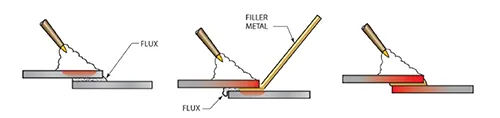
\includegraphics[width=0.8\linewidth]{soldering_brazing_welding.png} \footnote{\url{https://www.uti.edu/blog/welding/brazing-soldering-welding}}
\end{frame}
\begin{frame}{Review of Thermodynamics}
    \centering
    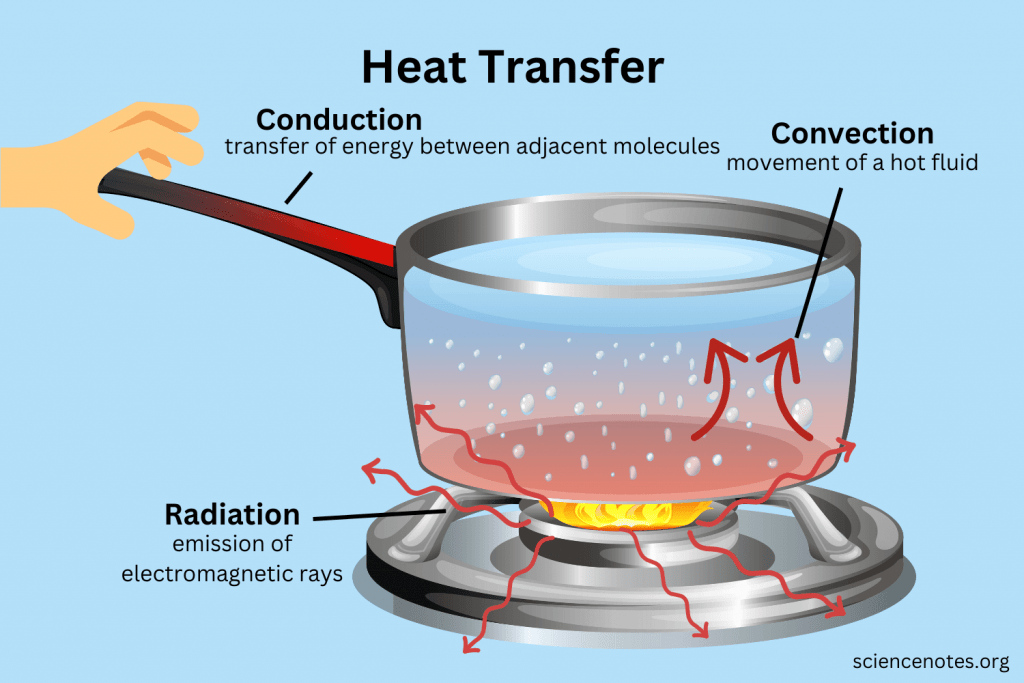
\includegraphics[height=0.8\textheight]{types_of_heat_transfer.png} \footnote{\url{https://sciencenotes.org/heat-transfer-conduction-convection-radiation/}}
\end{frame}
\begin{frame}{Fundamentals of Soldering}
    \begin{enumerate}
        \item Clean
        \item Tin
        \item Heat
        \item Flow
        \item Repeat
    \end{enumerate}
\end{frame}
\begin{frame}{Types of Soldering}
    \begin{itemize}
        \item Wire to Wire (low and high power)
        \item Wire/Through Hole to Connector/Board (low power)
        \item Wire to Board (high power)
        \item Surface Mount (exposed lead, no lead)
        \item Wire to Device (low power)
        \item Rework/Desoldering Through Hole
        \item Rework/Desoldering Surface Mount
    \end{itemize}
\end{frame}
\begin{frame}{Initial Training Scope}
    \begin{itemize}
        \item Wire to Wire (low power)
        \item Wire/Through Hole to Connector/Board (low power)
        \item Wire to Device (leaded coarse pitch)
    \end{itemize}
\end{frame}
\begin{frame}{Exercise \#1}
    Build a 22 AWG wire ring 1" in diameter
\end{frame}
\begin{frame}{Fundamentals of Soldering}
    \begin{enumerate}
        \item Clean
        \item Tin
        \item Heat
        \item Flow
        \item Repeat
    \end{enumerate}
\end{frame}
\begin{frame}{Exercise \#2}
    Solder D1, D2 on EK1950
\end{frame}
\begin{frame}{Fundamentals of Soldering}
    \begin{enumerate}
        \item Clean
        \item Tin
        \item Heat
        \item Flow
        \item Repeat
    \end{enumerate}
\end{frame}
\begin{frame}{Exercise \#3}
    Solder leads to JP1 on EK1950
\end{frame}
\begin{frame}{Fundamentals of Soldering}
    \begin{enumerate}
        \item Clean
        \item Tin
        \item Heat
        \item Flow
        \item Repeat
    \end{enumerate}
\end{frame}
\end{document}